\section{Applications for multibeam SEM}
\label{sec:5.2_mbsem}

For certain applications such as connectomics, in which the goal is to comprehensively reconstruct neuronal circuitry \cite{briggman2012volume}, fluorescence-based ROI targeting may be insufficient for limiting imaging volumes. The brains of small organisms, for example, can easily reach cubic millimeter volumes. Assuming \SI{5}{\nano\meter} isotropic pixel size (synaptic resolution), such volumes would take decades to image with a single electron beam due to limits on detector bandwidth and the amount of current that can be concentrated into a focused probe \cite{eberle2015high, kornfeld2018progress}. For this reason, a multibeam SEM, which scans in parallel by focusing multiple electron bundles onto a specimen, has long been a research topic in Delft \cite{zhang2008electron, mohammadi2013beams, ren2017imaging}, with an early adopter unit (FAST-EM, \cite{fermie2021high}) having recently been installed.

Despite its dramatic increases in imaging speeds, multibeam SEM bears the same limitation as conventional SEM with respect to the inability to provide inherent biological specificity. While for single beam SEM we addressed this problem by integrating a fluorescence microscope into the vacuum chamber, the same cannot be done for FAST-EM as sections are placed on a (nontransparent) scintillator substrate, the light from which serves as the detection mechanism. Alternatively, biological specificity could be added artificially (Fig \ref{fig:5.1_mbsem}). This could be done by preparing the same specimen for both FAST-EM and integrated array tomography. After initial processing of the specimen, the vast majority of serial sections would be placed onto a scintillator substrate for FAST-EM, while a small fraction ($\le$\,20) would be reserved for the integrated microscope. Following correlative imaging and reconstruction, the datasets would be used for training CLEMnet to predict on FAST-EM data. We have already seen that CLEMnet is capable of generating predictions on EM data acquired with different imaging settings than it was trained on (Section \ref{fig:4.4_robustness}). Early results have indicated that CLEMnet has the potential to generate fluorescence predictions on optical STEM data as well, given minor image processing augmentations \cite{abels2022}.

% Figure 5.1 (MB-SEM)
% -------------------
\begin{figure}[!tbh]
    \centering
    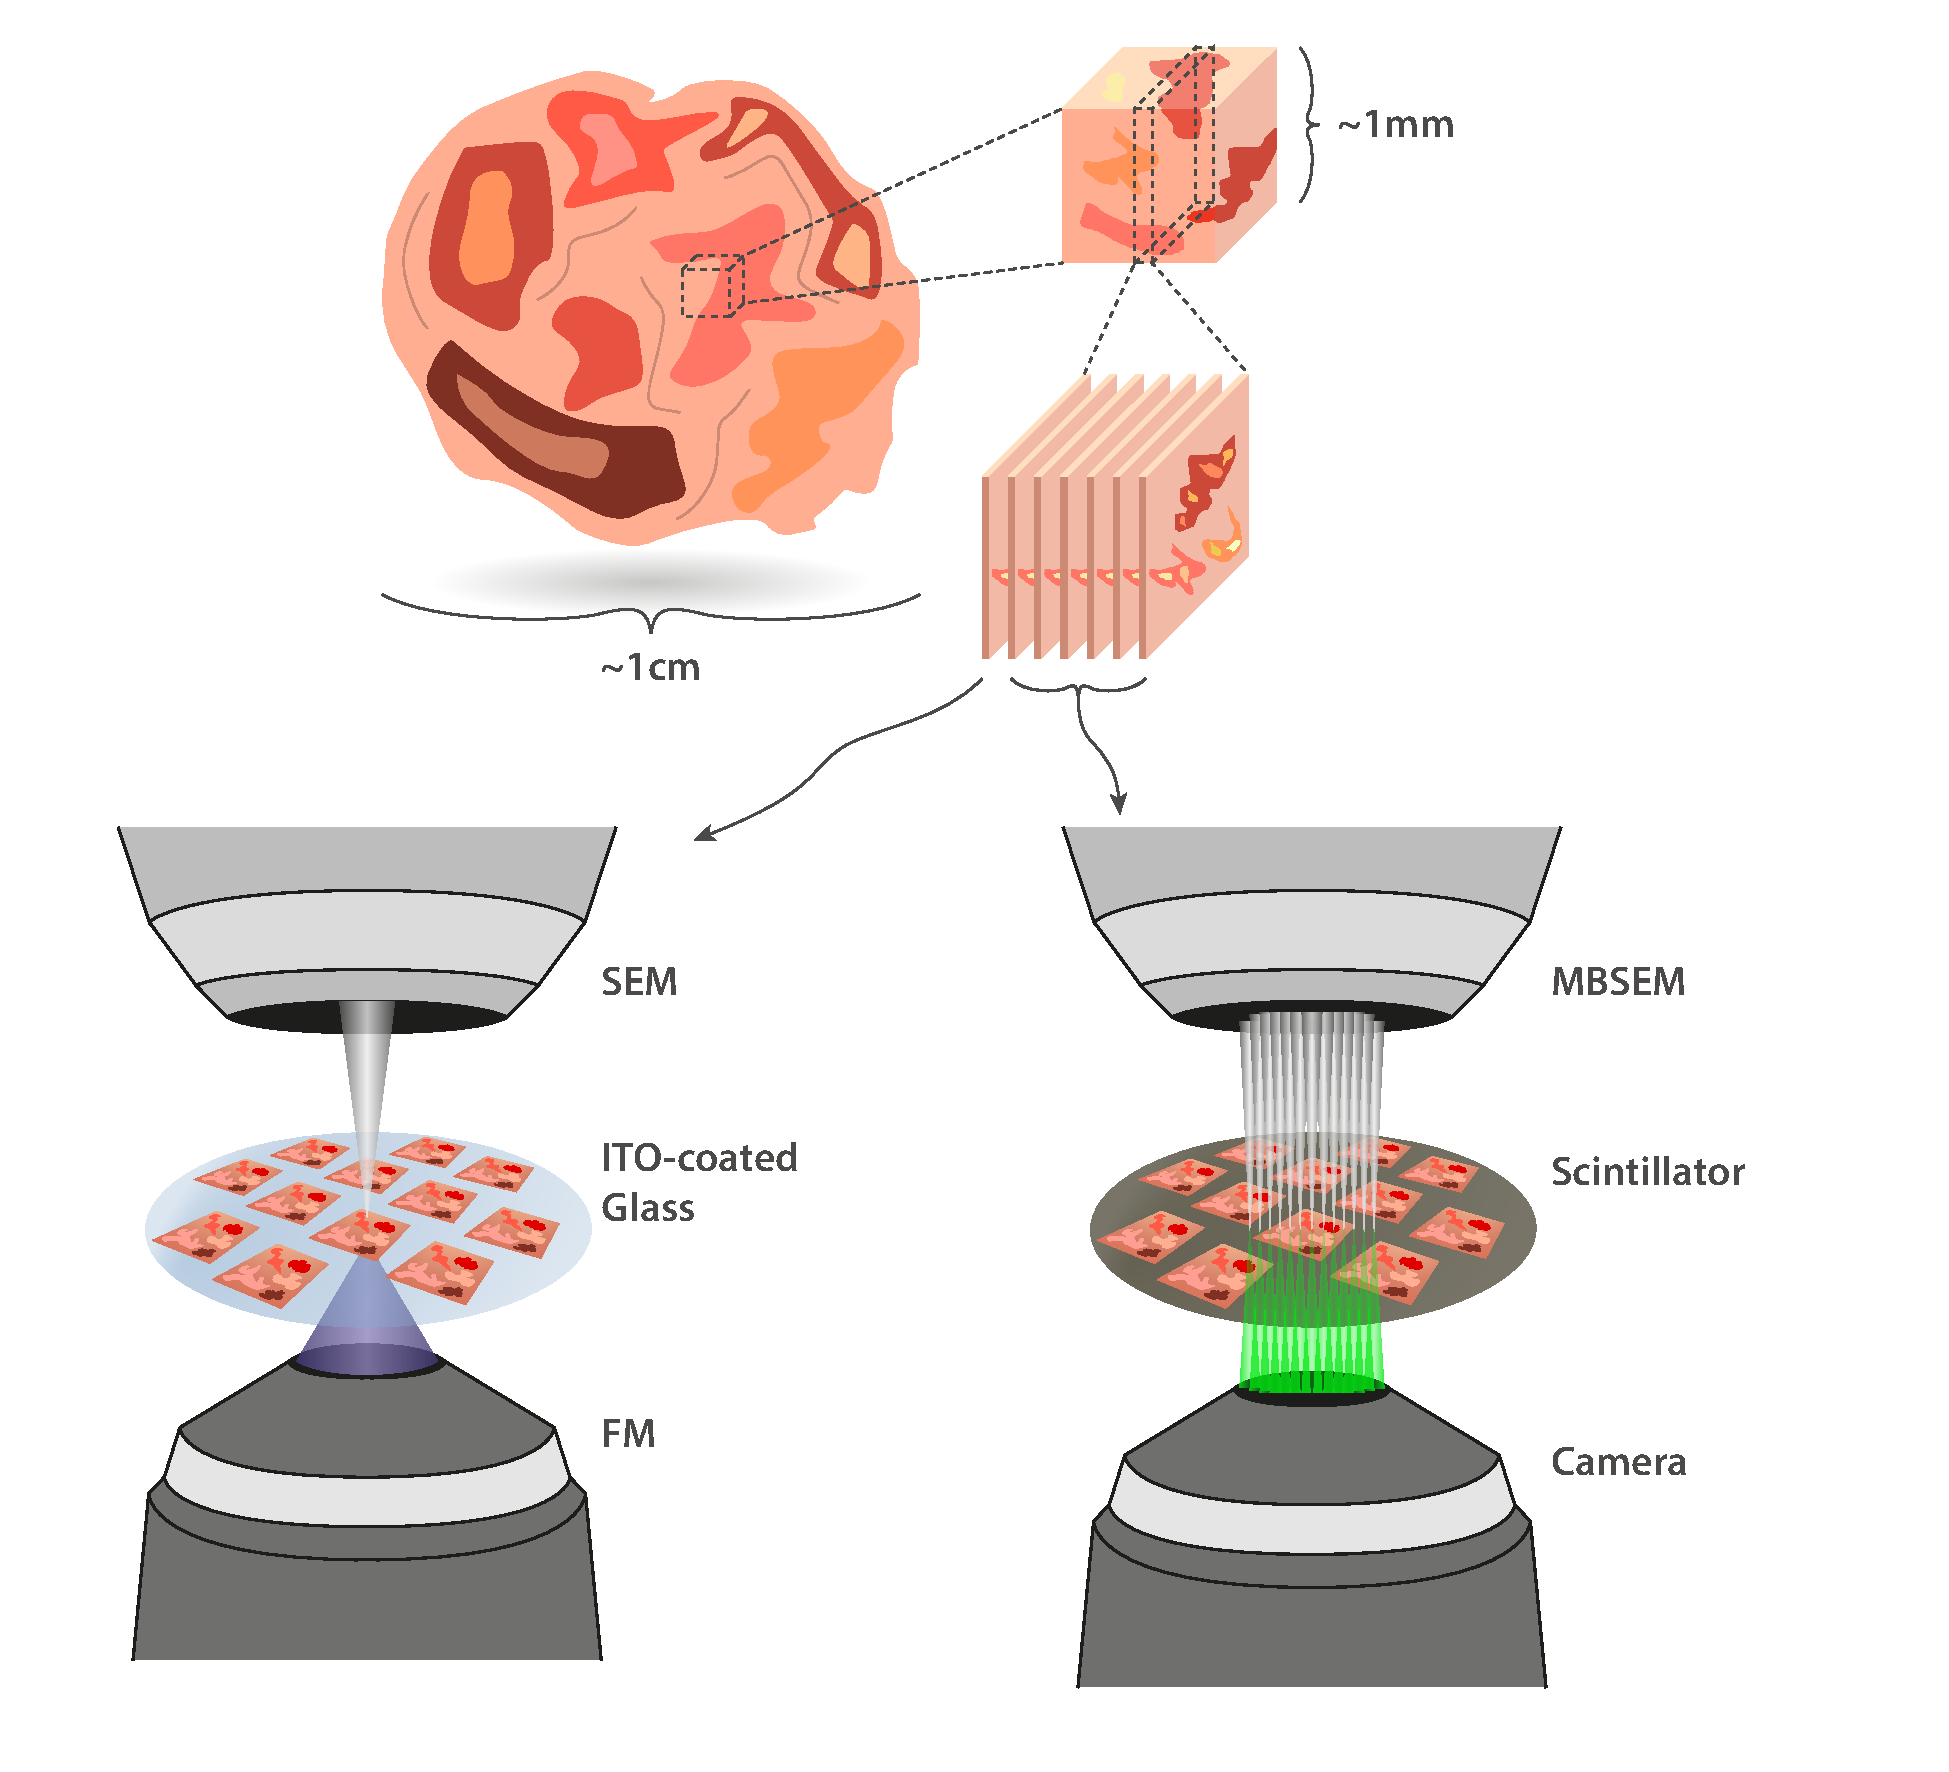
\includegraphics[width=\linewidth]{chapter-5/figures/multibeam_v1.pdf}
    \caption{Prospective workflow for adding artificial fluorescence to multibeam SEM data. Ultrathin sections are prepared for EM with the vast majority placed on a scintillator substrate to be imaged by multibeam SEM, while a small fraction of sections are placed onto ITO-coated glass for integrated CLEM.
    \textbf{TODO: Add neural network stuff? Where does the light from the scintillator actually go? A lens, camera or something else? Clean it up a bit, messy annotations, instruments have different heights, section count probably shouldn't be equal. MBSEM-->FAST-EM and ITO-coated glass --> ITO}}
    \label{fig:5.1_mbsem}
\end{figure}

There are, however, caveats to this approach that must be taken into consideration. First, there is no concrete means of verifying the fluorescence prediction as there is no measured fluorescence to serve as ground truth. Less precise verification methods do exist such as validating the predictions on sections adjacent to those for which the fluorescence was recorded. This may only be reliable, however, for structures significantly larger than the section thickness (e.g. cell nuclei, but not mitochondria, lysosomes, or granules). An alternative approach would be to manually segment the labelled structures in a subset of the FAST-EM data to establish a quasi-ground truth set for assessing the accuracy of the prediction. Another caveat is that there will be sections missing from the FAST-EM imaging volume due to the transfer of sections to ITO-coated glass. However, because the transferred sections will still be imaged with (single beam) SEM, they can be inserted into the image stack for 3D reconstruction, provided they are imaged at the same resolution.
